\section{Iterations}

The following five prototype iterations shown on figure \ref{fig:v1} to \ref{fig:v5}, depict an exploded view of the design on the left, and the physical version on the right. There is one major change in design during the process from prototype two to three, but they have all one thing in common: the journal is meant to be fixed on top of an acrylic sheet. \\

The first two prototype ideas shown on figures \ref{fig:v1} and \ref{fig:v2} were made entirely with acrylic sheets cut with a laser-cutter. The first prototype on figure \ref{fig:v1} was designed to accommodate eight banks of 4 x 1,5V AAA batteries. Compartments for each electronic component were made to place them on a flat surface, and reduce thickness. A box on the left of the journal was meant to hold LEDs. This design had many flaws however -- the list below describes the various issues.

\begin{itemize} \itemsep0em
  \item It felt heavy, and the weight exceeded 500g.
  \item The sharp edges from the laser-cut acrylic were slightly uncomfortable.
  \item The sheets were glued together, and made it impossible to open in case of the need for maintenance.
  \item The glueing process is tedious, because of of the use of extra tools such as a clamp, and the hardening takes 24h.
  \item Compartments were engraved with the laser-cutter, which requires constant supervision of the cutting.
  \item Problems with displacement of compartments from the different acrylic sheets.
  \item No charging possibility.
  \item Wiring of components was difficult.
  \item The side piece made it difficult to open the journal.
\end{itemize}

A few positive characteristics were observed:
\begin{itemize} \itemsep0em
  \item Removal of protruding bolts.
  \item Reduced thickness by 15mm.
\end{itemize}


\begin{figure}[h]
\begin{minipage}[b]{7.5cm}
\centering
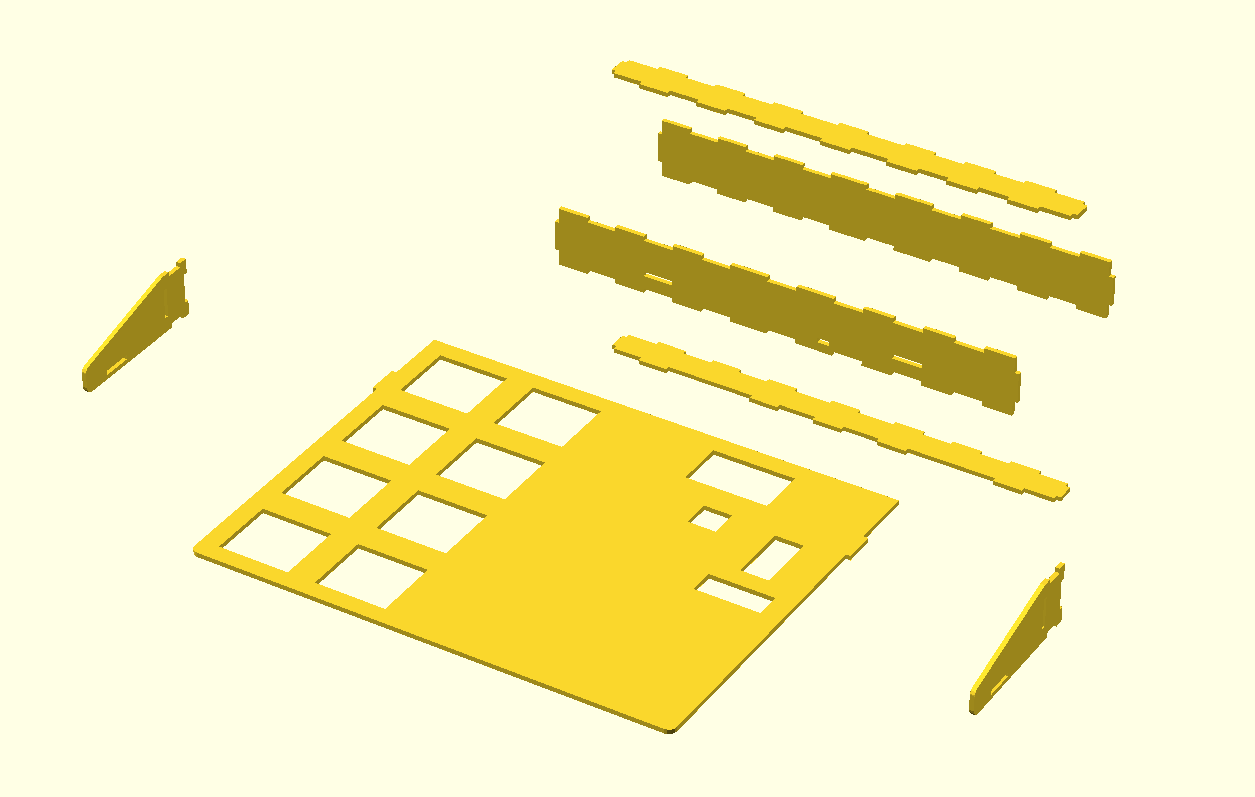
\includegraphics[scale=0.235]{figures/iterations/v1.png}
\end{minipage}
% \hspace{0.5cm}
\begin{minipage}[b]{7.5cm}
\centering
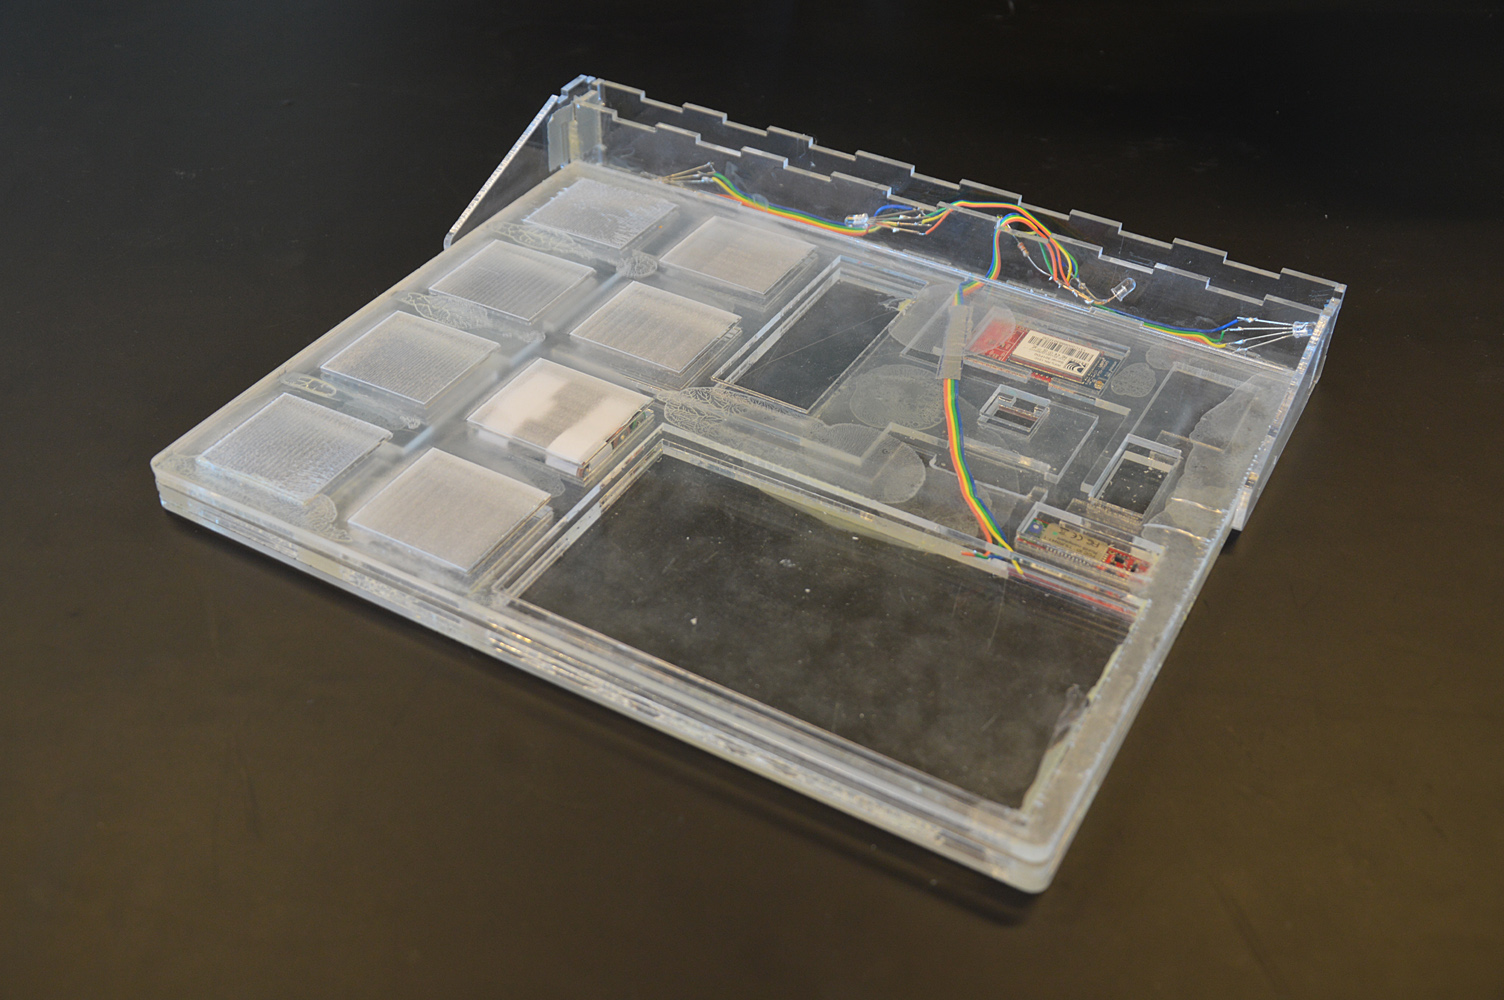
\includegraphics[scale=0.58]{figures/iterations/v1-photo.jpg}
\end{minipage}
\caption{\small {\it {The first prototype idea}}} \label{fig:v1}
\end{figure}

\clearpage

% -------------------

The second prototype took the previous downsides into consideration, and produced the device shown on figure \ref{fig:v2}. The idea here, is that the electronics were to be moved to a box at the bottom of the journal, in order to make the journal feel less bulky while holding it. \\

Following are the issues found with this design.

\begin{itemize} \itemsep0em
	\item Not very pleasant to hold, as the box holding the electronics ended up getting in the way of the user.
	\item Impossibility of performing maintenance, due to the acrylic being glued.
	\item Structurally unsound design - attachment of box to the sheet was flimsy, and broke easily.
	\item No charging possibility.
	\item The weight distribution would have been very uneven, due to the placement of box at the bottom.
\end{itemize}

\begin{figure}[h]
\begin{minipage}[b]{7.5cm}
\centering
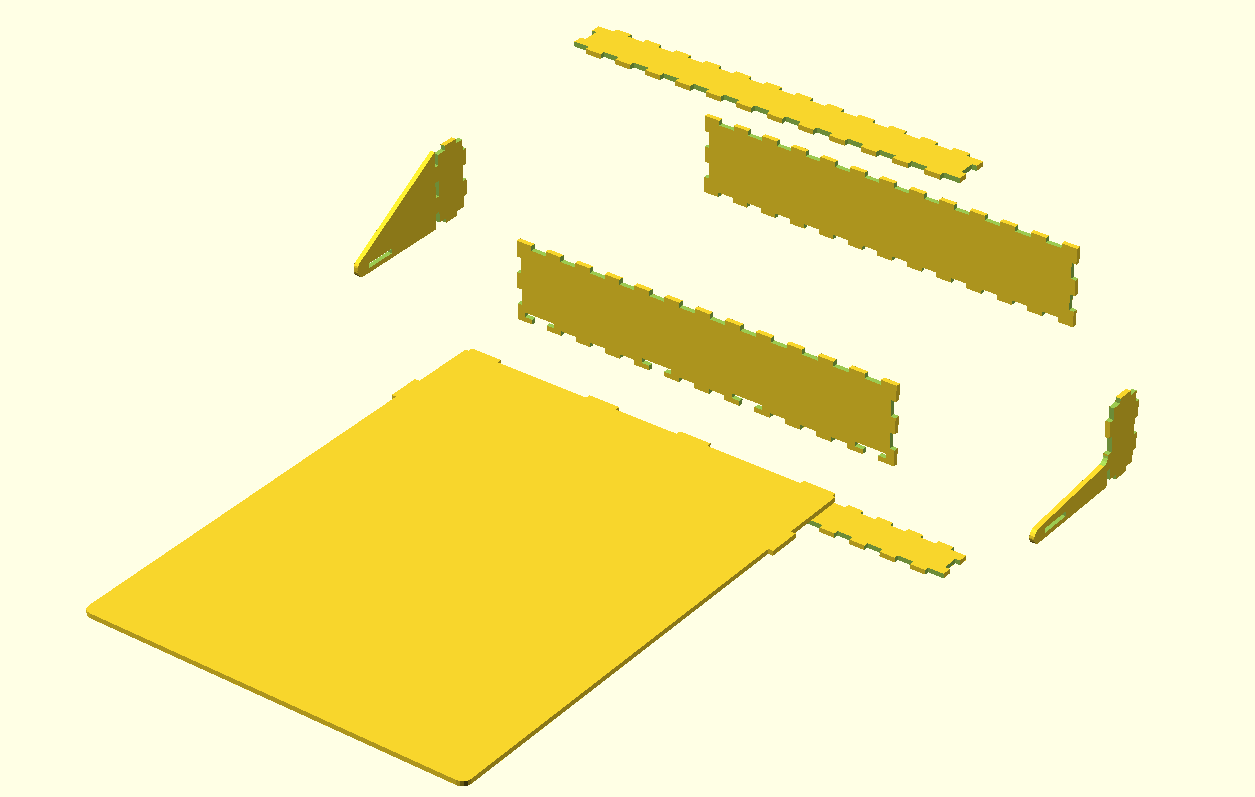
\includegraphics[scale=0.235]{figures/iterations/v3.png}
\end{minipage}
% \hspace{0.5cm}
\begin{minipage}[b]{7.5cm}
\centering
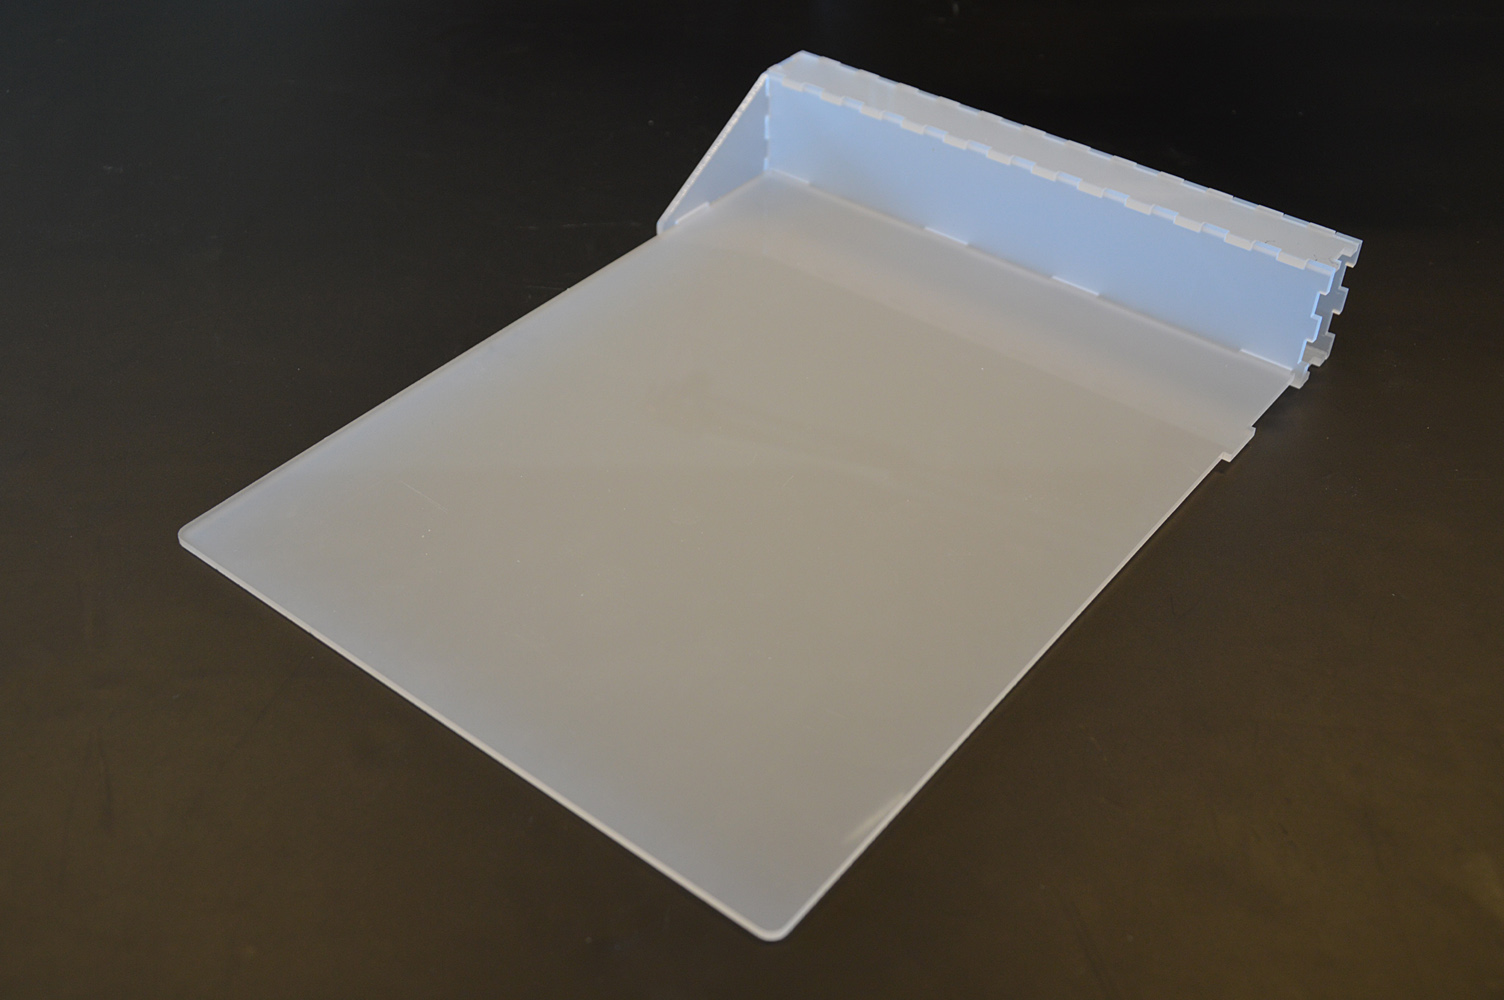
\includegraphics[scale=0.58]{figures/iterations/v3-photo.jpg}
\end{minipage}
\caption{\small {\it {The second prototype idea}}} \label{fig:v2}
\end{figure}

This prototype was discarded before an attempt to place the electronics in the box, due to the obvious disadvantages. The technique of laser-cutting acrylic sheets and using glue to attach them together proved to be a slow and tedious task. Due to the difficulty of using screws to assemble the parts and using glue instead, made the designs unmaintainable. Complex laser-cut acrylic parts also tended to become brittle, so a rethinking of the design was in order. Using acrylic wasn't out of the question, but the complexity of those parts had to be reduced, and the use of 3D printed PLA for those parts were introduced in the following prototype. \\

% -------------------

\begin{figure}[h]
\begin{minipage}[b]{7.5cm}
\centering
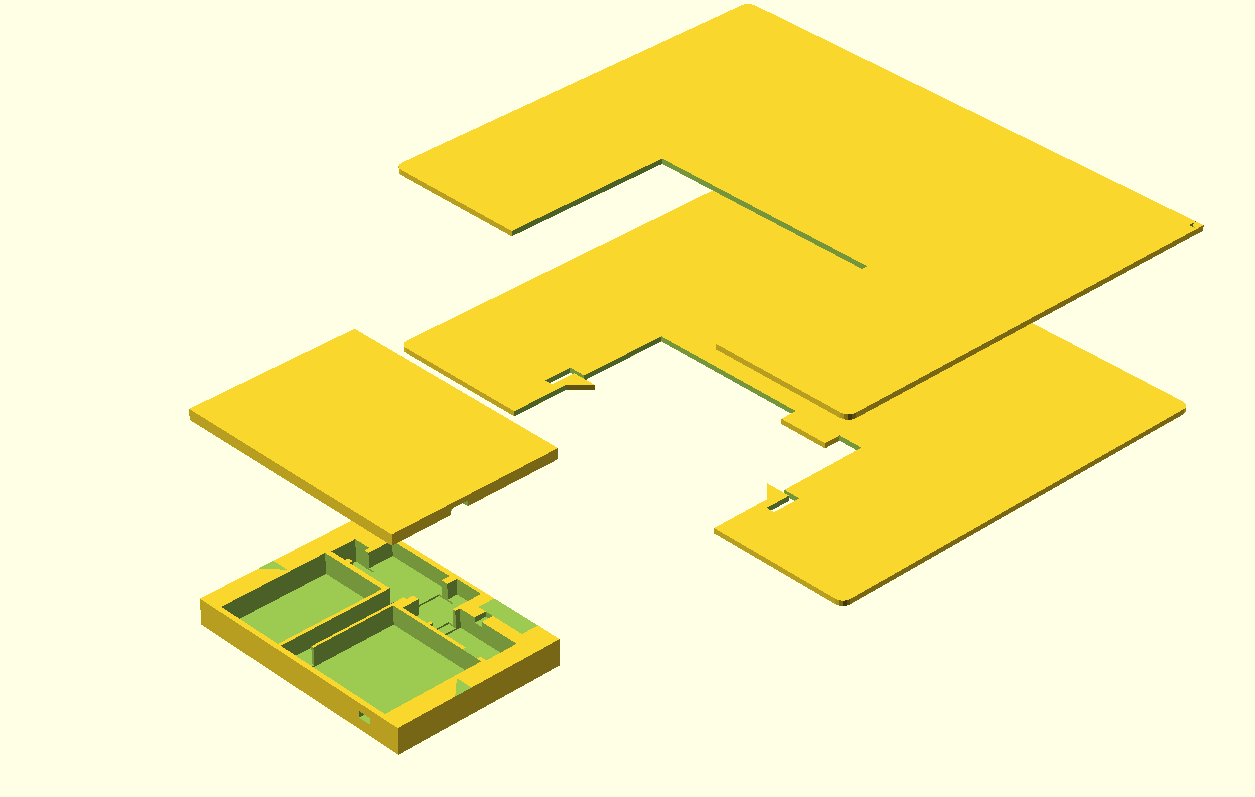
\includegraphics[scale=0.235]{figures/iterations/v4.png}
\end{minipage}
% \hspace{0.5cm}
\begin{minipage}[b]{7.5cm}
\centering
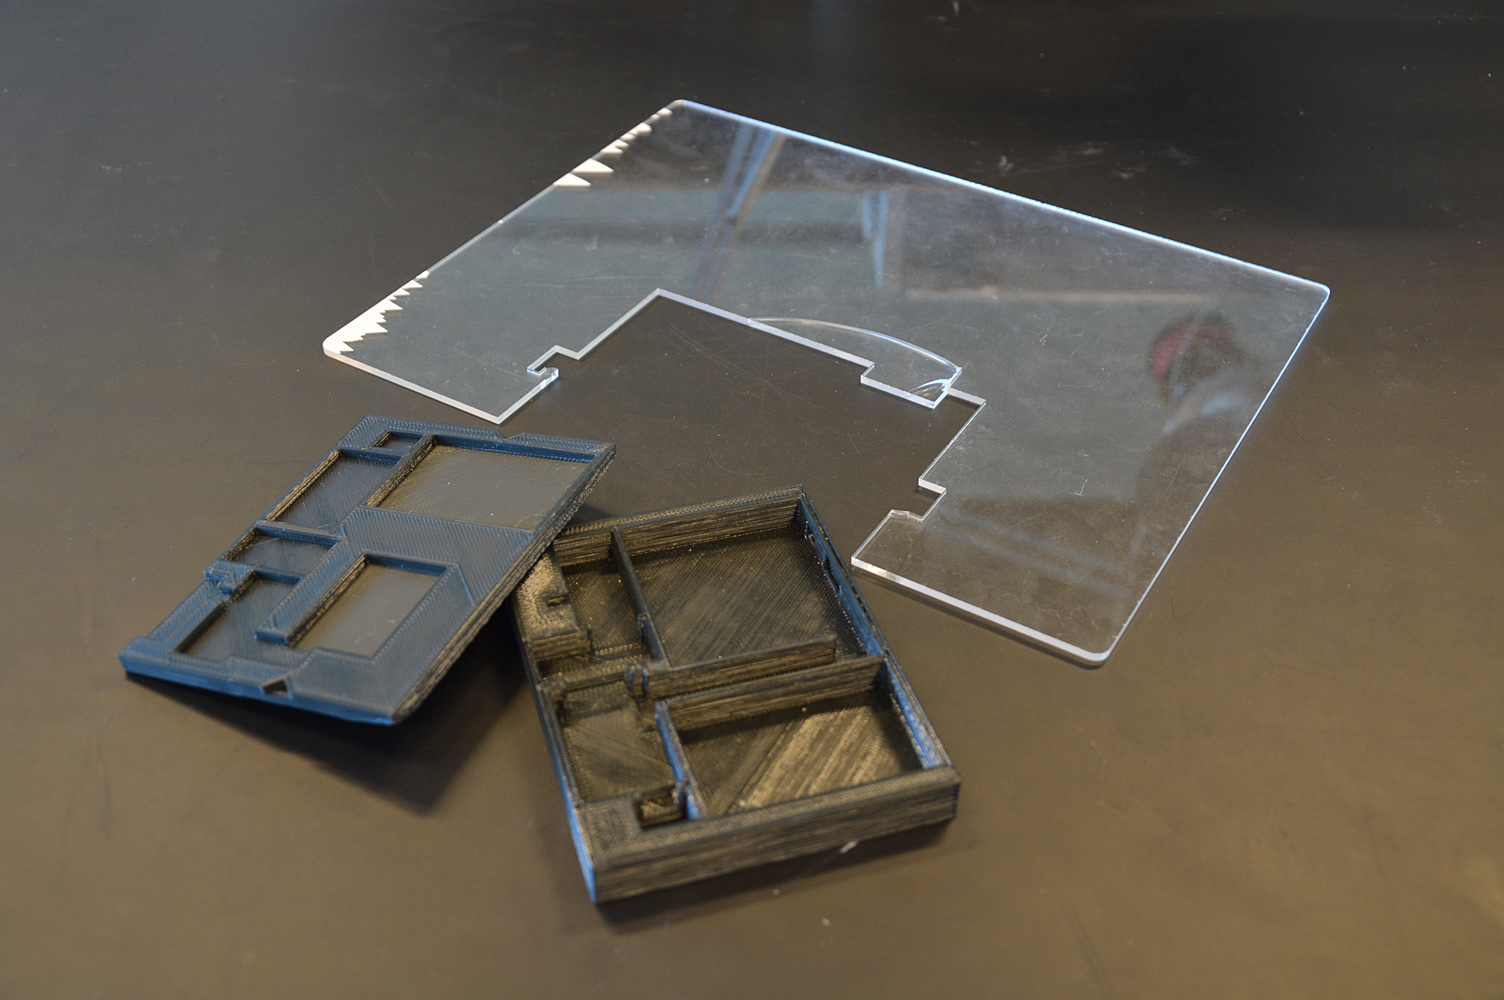
\includegraphics[scale=0.58]{figures/iterations/v4-photo.jpg}
\end{minipage}
\caption{\small {\it {The third prototype idea}}} \label{fig:v3}
\end{figure}

The third prototype was different from the two previous. Figure \ref{fig:v3} depicts the design. The electronics was moved to a new 3D printed container, made of PLA. The latter was further divided into smaller compartments, made for housing the various electronic components. The box was also designed to be slid into a sheet of acrylic. Two small protruding triangles where cut in order for them to bend, and the box would then ``click'' into place. This was however difficult to get right, and the bending acrylic ended up breaking quickly. Figure \ref{fig:v3} shows the broken acrylic on the right. A second sheet of acrylic was added,



% -------------------

\begin{figure}[h]
\begin{minipage}[b]{7.5cm}
\centering
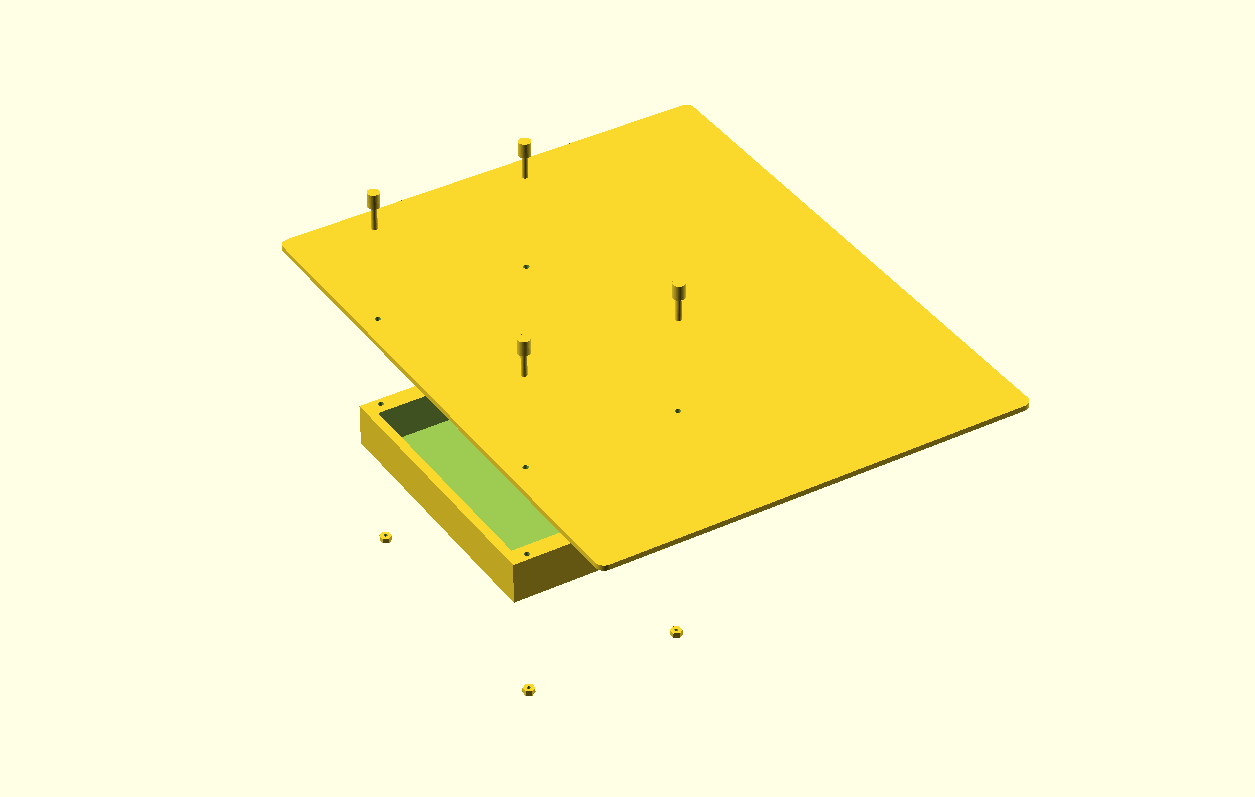
\includegraphics[scale=0.235]{figures/iterations/v5.png}
\end{minipage}
% \hspace{0.5cm}
\begin{minipage}[b]{7.5cm}
\centering
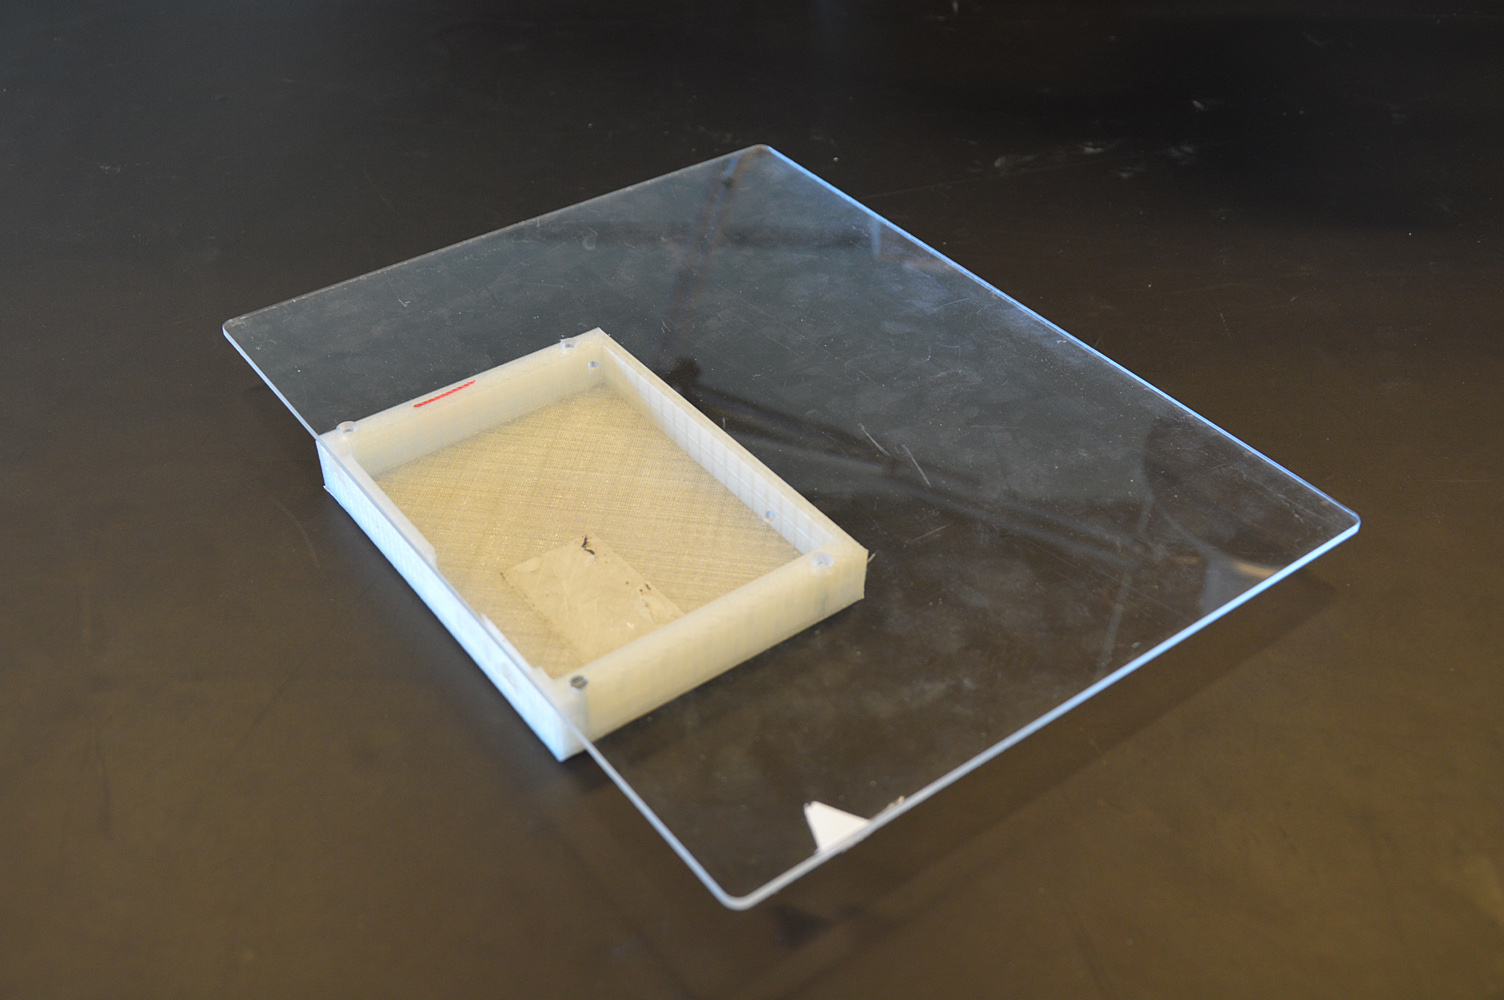
\includegraphics[scale=0.58]{figures/iterations/v5-photo.jpg}
\end{minipage}
\caption{\small {\it {The fourth prototype idea}}} \label{fig:v4}
\end{figure}

% -------------------

\begin{figure}[h]
\begin{minipage}[b]{7.5cm}
\centering
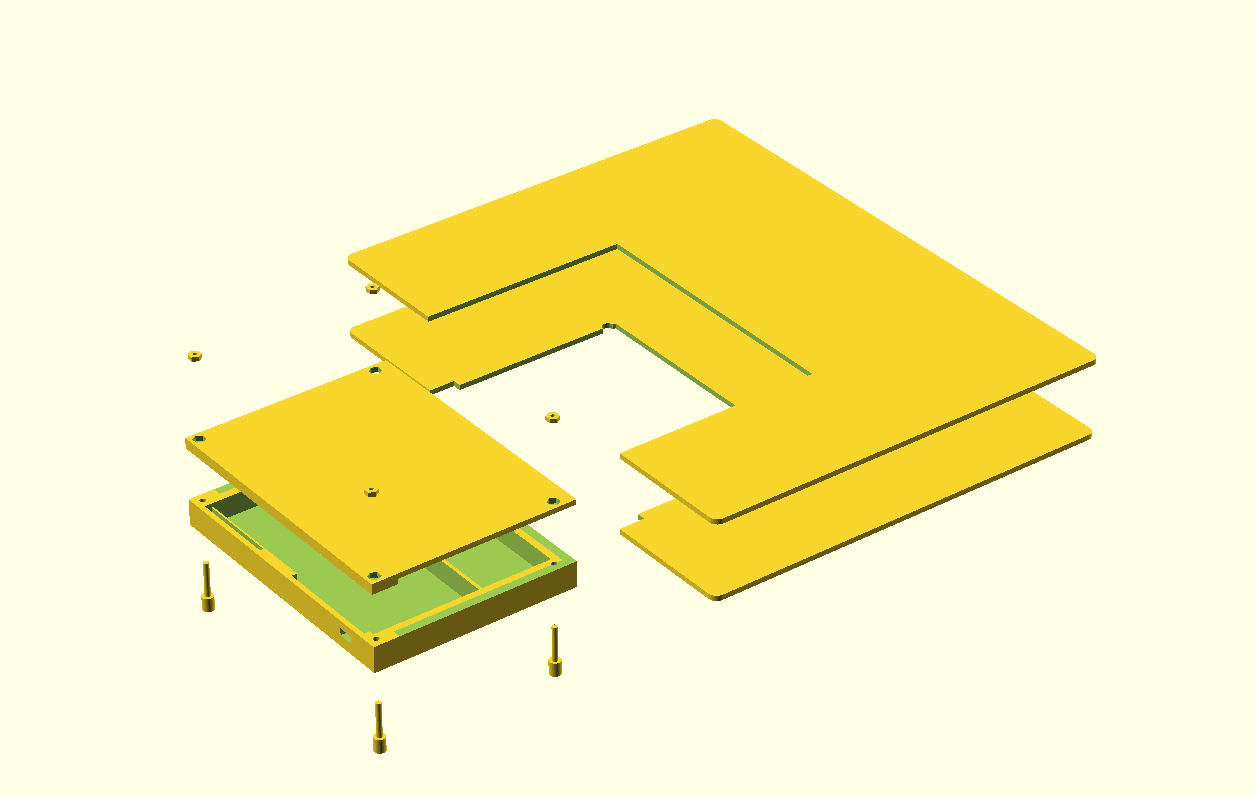
\includegraphics[scale=0.235]{figures/iterations/v6.png}
\end{minipage}
% \hspace{0.5cm}
\begin{minipage}[b]{7.5cm}
\centering
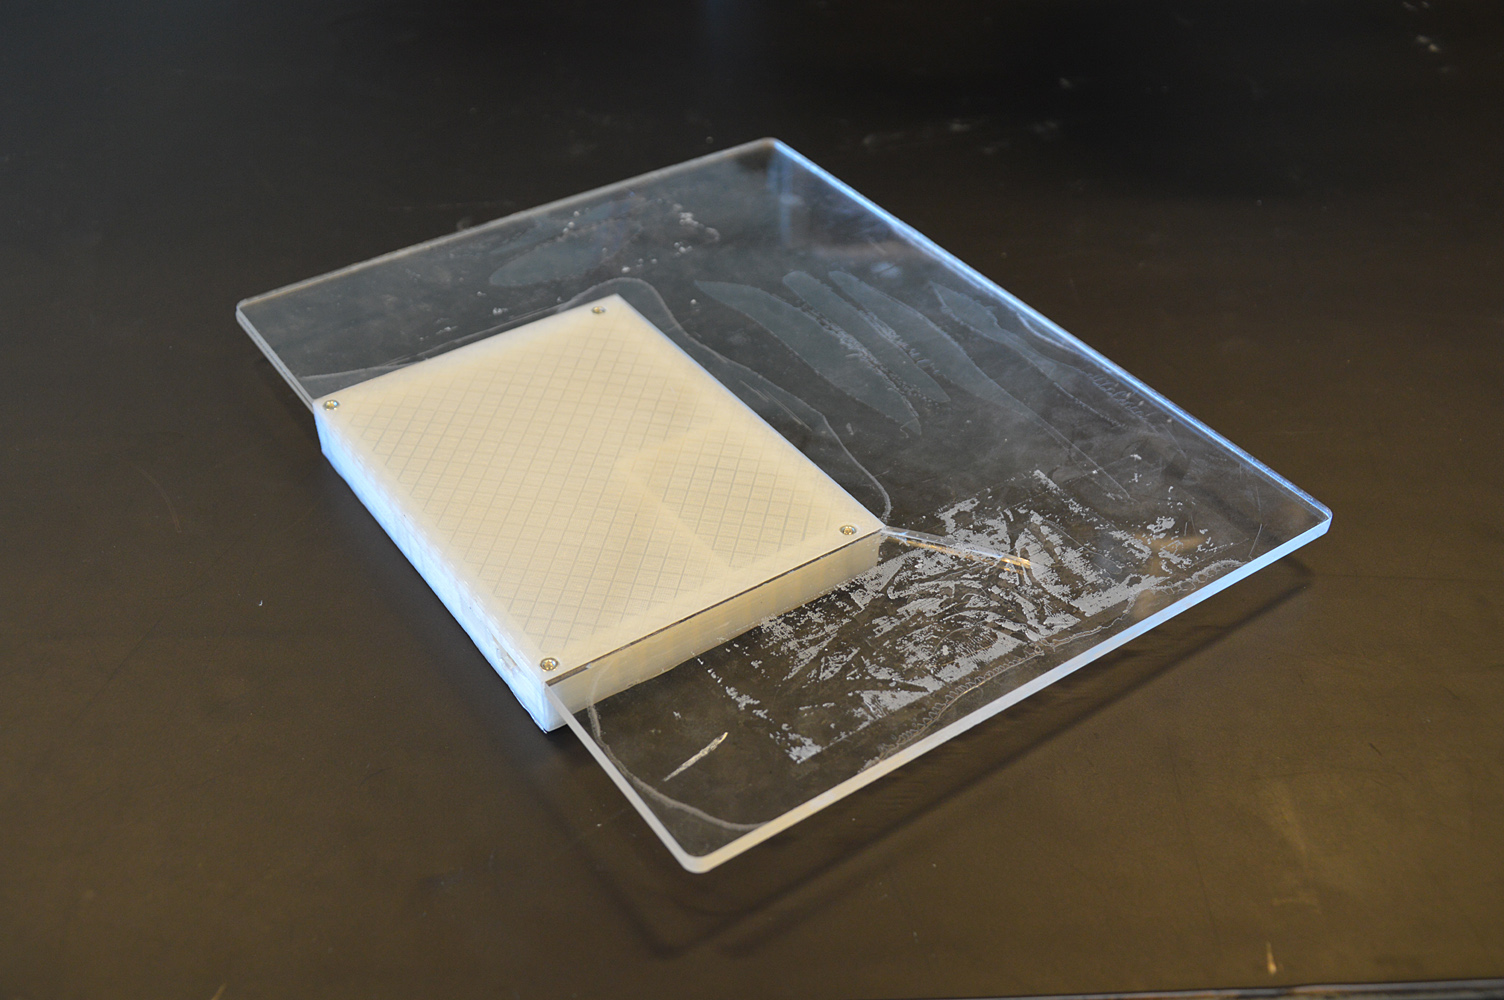
\includegraphics[scale=0.58]{figures/iterations/v6-photo.jpg}
\end{minipage}
\caption{\small {\it {The fifth prototype idea}}} \label{fig:v5}
\end{figure}

% -------------------

\clearpage